
\section{指定绘制范围}

\subsection{界限范围的配置}

\begin{pgfplotsxykeylist}{%
    \x min=\marg{coord},
    \x max=\marg{coord},
    min=\marg{coord},
    max=\marg{coord}%
}
\labelprefix\label{page:access:limits}
    这些选项用于定义坐标轴界限，即左下角和右上角。坐标轴界限之外的所有内容都将被裁剪掉。


    \paragraph{注意：}

    这些值（以及本节中其他相关键）仅影响 \PGFPlots{} 如何确定坐标轴范围。这些值与函数采样\emph{无关}。请参阅 |domain| 以定义绘图表达式的采样范围。采样范围大于或小于坐标轴的显示部分都是允许的。使用 |xmin| 及其同类键来指定坐标轴的哪一部分需要显示。

    这些键中的每一个都是可选的，缺失的界限将根据输入数据自动确定。这里，|min| 和 |max| 键将 $x$、$y$ 和 $z$ 的界限设置为相同的 \meta{coord}。

    如果已显式指定 $x$ 界限而 $y$ 界限自动计算，则 $y$ 界限的自动计算将只考虑落入指定 $x$ 范围内的点（反之亦然）。例如，如果只显式提供了 |xmin|，情况同样如此：在那种情况下，|xmax| 将只针对满足 $x \ge \;$|xmin| 的点进行更新。可以使用 |clip limits=false| 禁用此功能。

    坐标轴界限可以使用 |enlargelimits| 选项自动增大。
    %
\begin{codeexample}[]
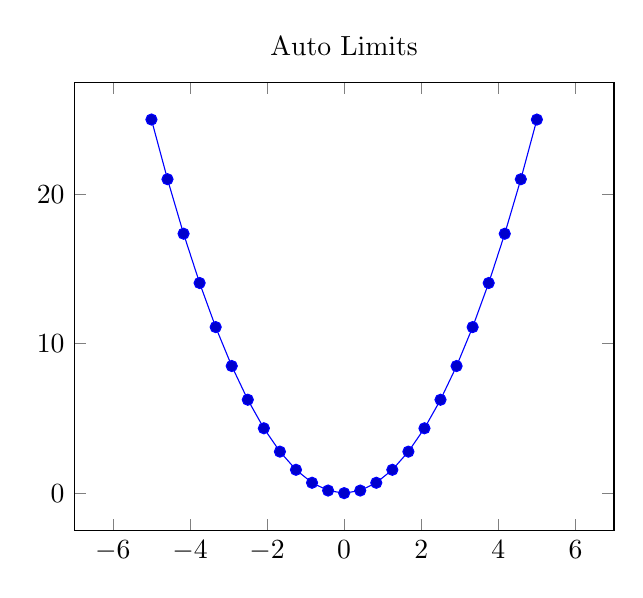
\begin{tikzpicture}
\begin{axis}[
    title=Auto Limits,
]
    \addplot {x^2};
\end{axis}
\end{tikzpicture}
\end{codeexample}

\begin{codeexample}[]
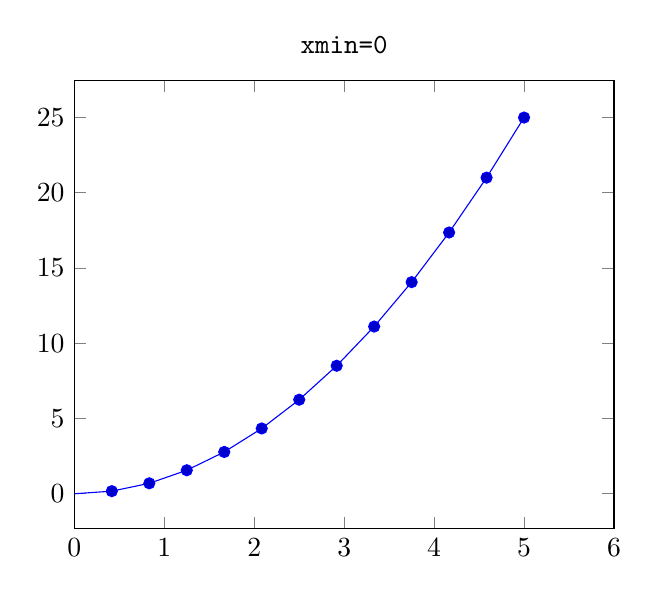
\begin{tikzpicture}
\begin{axis}[
    title={\texttt{xmin=0}},
    xmin=0,
]
    \addplot {x^2};
\end{axis}
\end{tikzpicture}
\end{codeexample}

\begin{codeexample}[]
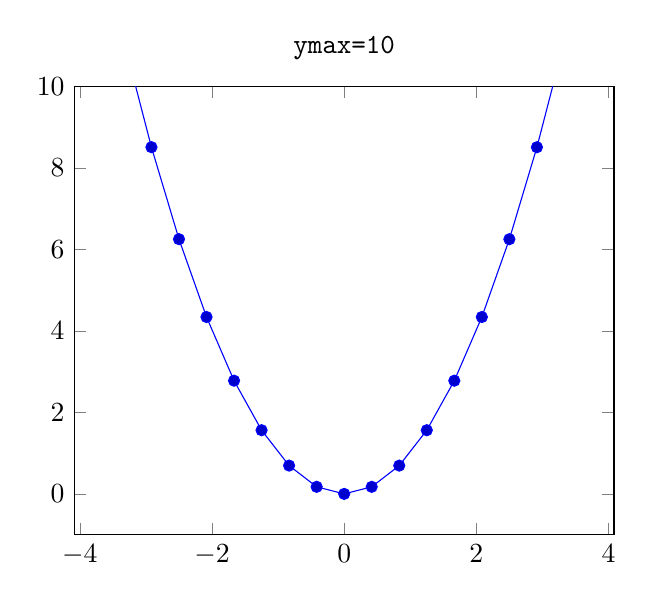
\begin{tikzpicture}
\begin{axis}[
    title={\texttt{ymax=10}},
    ymax=10,
]
    \addplot {x^2};
\end{axis}
\end{tikzpicture}
\end{codeexample}

    请注意，即使你提供 |ymax=10|，$y>10$ 的数据点仍会被绘制出来——从而产生一条超出绘制范围的线。

    另请参阅 |restrict x to domain| 和 |restrict x to domain*| 键——它们分别允许丢弃或裁剪位于某个定义域之外的输入坐标。

    在可视化阶段，即在 |\end{axis}| 处，这些键将被设置为最终的坐标轴界限。你可以通过 |\pgfkeysvalueof{/pgfplots/xmin}| 来访问这些值，例如：
    %
\begin{codeexample}[]
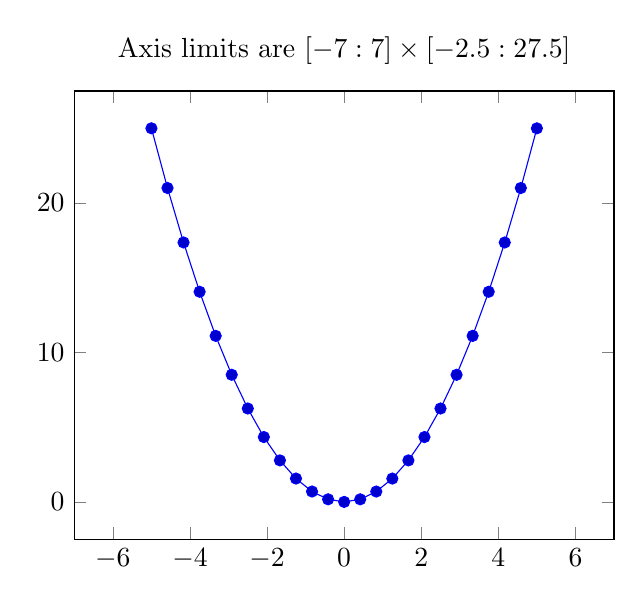
\begin{tikzpicture}
\begin{axis}[
 % Show (automatically) computed limits:
 title={
  Axis limits are
  $
 [\pgfmathprintnumber{\pgfkeysvalueof{/pgfplots/xmin}}
 :\pgfmathprintnumber{\pgfkeysvalueof{/pgfplots/xmax}}
 ]  \times
 [\pgfmathprintnumber{\pgfkeysvalueof{/pgfplots/ymin}}
 :\pgfmathprintnumber{\pgfkeysvalueof{/pgfplots/ymax}}
 ]$ },
]
    \addplot {x^2};
\end{axis}
\end{tikzpicture}
\end{codeexample}
    %
    这种访问在任何坐标轴描述（如 |xlabel|、|title|、|legend entries| 等）或任何注释（即在 |\node|、|\draw| 或 |\path| 内部以及 |(|\meta{x}|,|\meta{y}|)| 形式的坐标）中都是可行的，但在 |\addplot| 内部不行（在此阶段界限可能尚未完整）。
\end{pgfplotsxykeylist}

\begin{pgfplotsxykey}{\x mode=\mchoice{normal,linear,log} (initially normal)}
    允许为每个 $x,y,z$ 组合选择线性（即 normal）或对数坐标轴缩放，或对数图。

    对数图使用 |log basis x| 及其变体的当前设置来确定底数（默认为 $e$）。
    % FIXME : replicated in pgfplots.reference.scaling.tex
\end{pgfplotsxykey}

\begin{pgfplotsxykey}{\x\ dir=\mchoice{normal,reverse} (initially normal)}
\labelprefix\label{key:pgfplots:xydir}%
\pgfkeys{/pdflinks/search key prefixes in/.add={/pgfplots/,}{}}
    允许反转坐标轴方向，使值按递减顺序给出。
    %
\begin{codeexample}[]
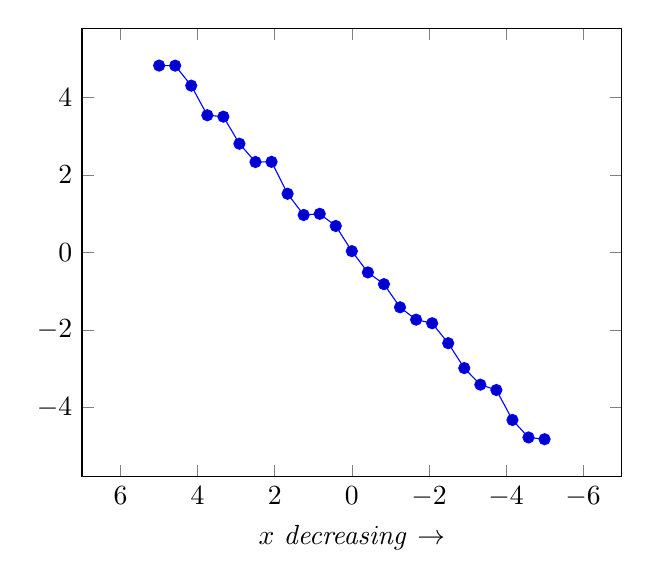
\begin{tikzpicture}
\begin{axis}[
    xlabel=$x$ \emph{decreasing} $\to$,
    x dir=reverse,
]
    \addplot {x + rand*0.3};
\end{axis}
\end{tikzpicture}
\end{codeexample}

\begin{codeexample}[]
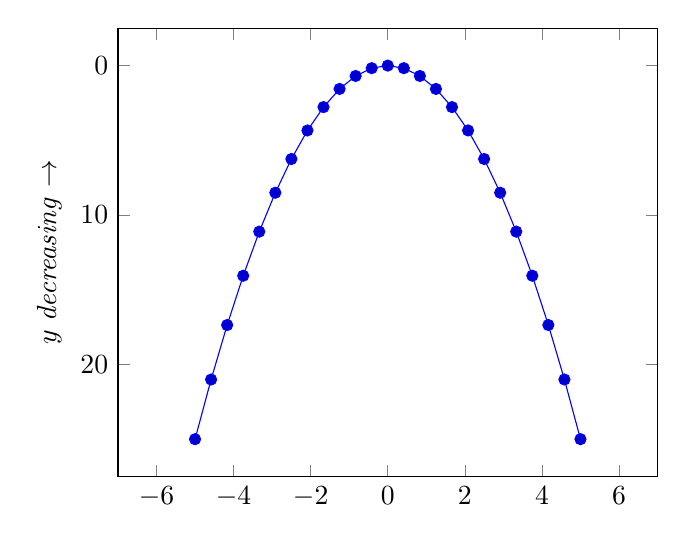
\begin{tikzpicture}
\begin{axis}[
    ylabel=$y$ \emph{decreasing} $\to$,
    y dir=reverse,
]
    \addplot {x^2};
\end{axis}
\end{tikzpicture}
\end{codeexample}

    请注意，坐标轴描述和相对定位宏将保持在与未反转坐标轴时相同的位置。
    %
\begin{codeexample}[]
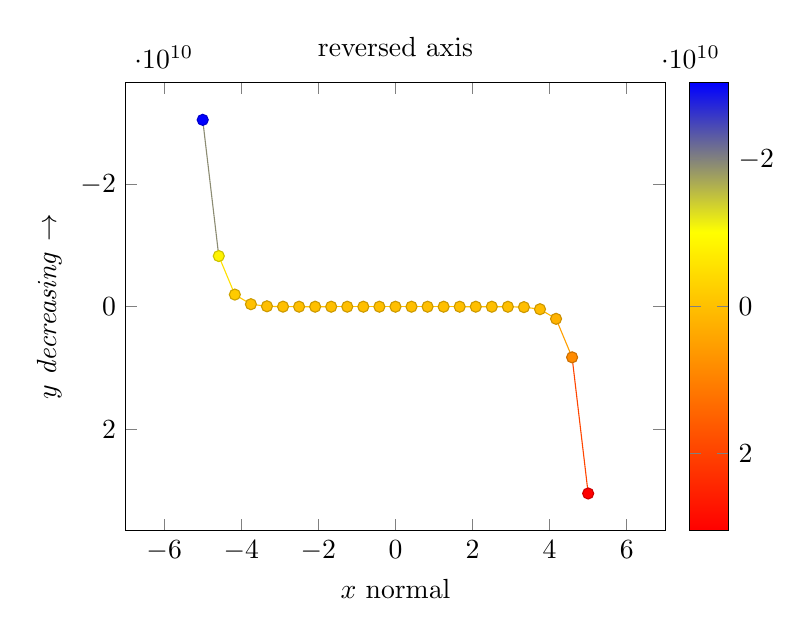
\begin{tikzpicture}
    \begin{axis}[
        ylabel=$y$ \emph{decreasing} $\to$,
        xlabel=$x$ normal,
        title=reversed axis,
        y dir=reverse,
        colorbar,
        colorbar style={y dir=reverse},
    ]
        \addplot+ [mesh,scatter] {x^15};
    \end{axis}
\end{tikzpicture}
\end{codeexample}

    请注意，|colorbar| 不会自动反转；如果需要（如前例所示），你必须手动反转颜色条的序列。
\end{pgfplotsxykey}

\begin{pgfplotsxykeylist}{clip \x limits=\mchoice{true,false} (initially true),clip limits=\mchoice{true,false}}
    配置当部分（但非全部）坐标轴界限被显式指定时应如何处理。在 |clip limits=true| 的情况下，自动界限计算将\emph{仅}考虑与显式设置的界限不矛盾的点。

    |clip xlimits=true| 的效果是：如果某个点 $(x,y)$ 的 $x$ 坐标落在由 |xmin| 和 |xmax| 指定的界限之外，则 $x$ 和 $y$ 都不会对自动计算的坐标轴界限产生贡献。键 |clip limits| 是一个别名，用于一次性设置所有其他选项。

    此选项与路径裁剪无关，它仅影响坐标轴界限的计算方式。
\end{pgfplotsxykeylist}

\begin{pgfplotsxykeylist}{%
    enlarge \x\ limits=\mchoice{%
        auto,
        true,false,
        upper,lower,
        \meta{val},value=\meta{val},
        abs value=\meta{val},\\ abs=\meta{val},
        rel=\meta{val}%
    } (initially auto),
    enlargelimits=\meta{common value}%
}
    启用时，会略微增大某一坐标轴（或对于 |enlargelimits| 为所有坐标轴）的尺寸。

    你可以将 |xmin|、|xmax| 和 |ymin|、|ymax| 设置为数据的最小/最大值，|enlarge x limits| 将放大画布，使坐标轴不接触图形。

    值 \declaretext{true} 会增大下限和上限。

    值 \declaretext{false} 使用用户指定的（或从输入坐标读取的）紧凑坐标轴界限。

    值 \declaretext{auto} 将仅为坐标轴界限被自动确定的坐标轴增大界限。对于三维图形，\declaretext{auto} 机制仅适用于 $z$ 轴。$x$ 轴和 $y$ 轴不会被增大。
    %
\begin{codeexample}[]
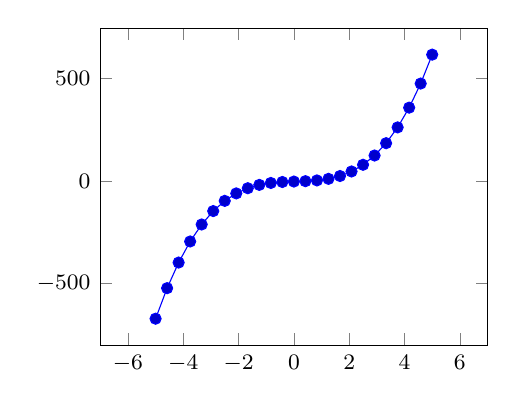
\begin{tikzpicture}
\begin{axis}[
    small,
]
    \addplot {5 * x^3 - x^2 + 4*x -2};
\end{axis}
\end{tikzpicture}
\end{codeexample}

     指定数字 \declaretext{val}ue，如 `|enlarge x limits=0.2|'，将相对地增大坐标轴的下限和上限。下面的示例在两侧各添加坐标轴界限的 $20\%$：
     %
\begin{codeexample}[]
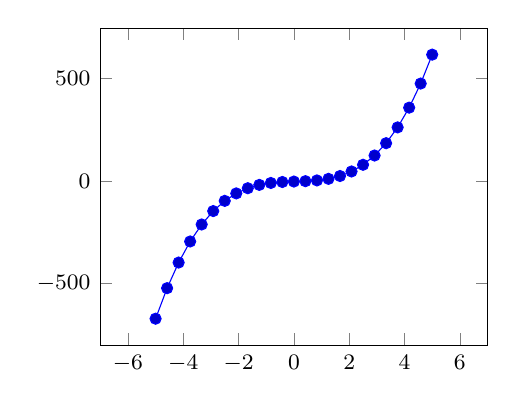
\begin{tikzpicture}
\begin{axis}[
    small,
    enlarge x limits=0.2,
]
    \addplot {5 * x^3 - x^2 + 4*x -2};
\end{axis}
\end{tikzpicture}
\end{codeexample}
    %
    \noindent 选项 \declaretext{rel=}\marg{value} 与 |true,value=|\marg{value} 相同，即它为 |upper| 和 |lower| 界限都激活相对增大。

    值 \declaretext{upper} 仅增大坐标轴上限，而 \declaretext{lower} 仅增大坐标轴下限。在这种情况下，添加到相应界限的量可以使用 \declaretext{value=}\marg{val} 键指定。它可以与任何其他可能的值组合。例如，

        |\pgfplotsset{enlarge x limits={value=0.2,upper}}|

    将（仅）把坐标轴上限增大坐标轴范围的 $20\%$。另一个例子是

        |\pgfplotsset{enlarge x limits={value=0.2,auto}}|

    它将 \declaretext{auto} 值的默认阈值更改为 $20\%$。
    %
\begin{codeexample}[]
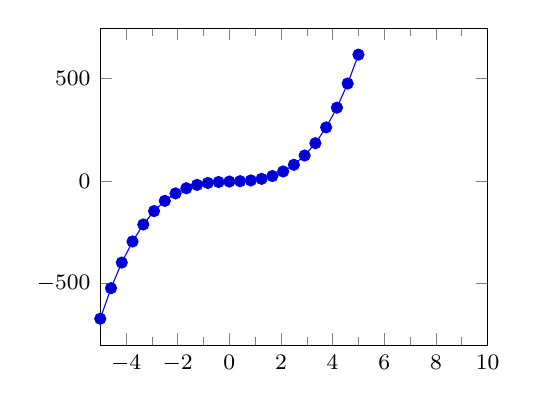
\begin{tikzpicture}
\begin{axis}[
    small,
    minor x tick num=1,
    enlarge x limits={rel=0.5,upper},
]
    \addplot {5 * x^3 - x^2 + 4*x -2};
\end{axis}
\end{tikzpicture}
\end{codeexample}

     虽然 |value| 使用相对阈值，但 \declaretext{abs value} 接受绝对值：它向所选坐标轴添加一个绝对值。选项 \declaretext{abs=}\marg{value} 与 |true,abs value=|\marg{value} 相同，即它向 |upper| 和 |lower| 界限都添加一个绝对值：
     %
\begin{codeexample}[]
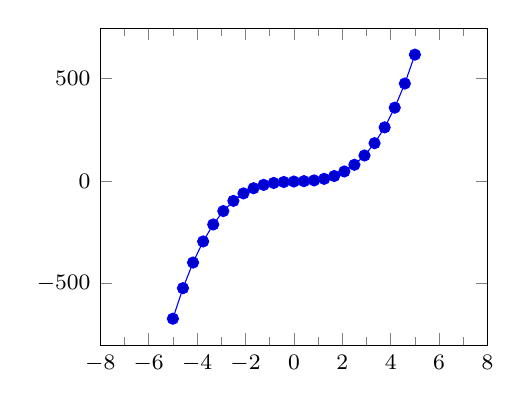
\begin{tikzpicture}
\begin{axis}[
    small,
    minor x tick num=1,
    enlarge x limits={abs=3},
]
    \addplot {5 * x^3 - x^2 + 4*x -2};
\end{axis}
\end{tikzpicture}
\end{codeexample}
    %
    \noindent 这里，我们将 $x$ 轴增大了 $3$ 个单位。请注意，你也可以指定 \emph{尺寸}，如 |1cm|：
    %
\begin{codeexample}[]
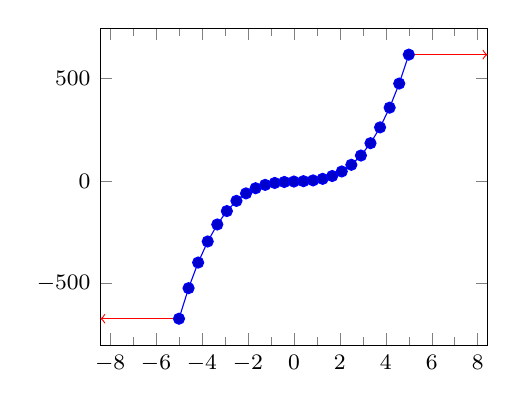
\begin{tikzpicture}
\begin{axis}[small,minor x tick num=1,
    enlarge x limits={abs=1cm},
]
    \addplot {5 * x^3 - x^2 + 4*x -2}
        coordinate [pos=0] (first)
        coordinate [pos=1] (last);

    \draw [red,->] (first) -- ++(-1cm,0pt);
    \draw [red,->] (last)  -- ++( 1cm,0pt);
\end{axis}
\end{tikzpicture}
\end{codeexample}
    %
    \noindent 从技术上讲，使用绝对尺寸略有不同。例如，它允许增大超过 |width| 的量，这对所有其他选项是不可能的。\PGFPlots{} 将尝试同时满足提供的 |width|/|height| 和绝对坐标轴增大。如果做不到，它将放弃 |width|/|height| 约束，并向日志文件打印一条警告消息。另请参阅键 |enlargelimits respects figure size|。
    \index{Errors!enlargelimits respects figure size=true: could not respect the prescribed width/height}


    \paragraph{注意：}

    对于对数坐标轴，|abs value| 是以\emph{乘法方式}应用的！这意味着对于对数坐标轴，|abs value=10| 会向上限和/或下限添加 $\log 10$。
    %
\begin{codeexample}[]
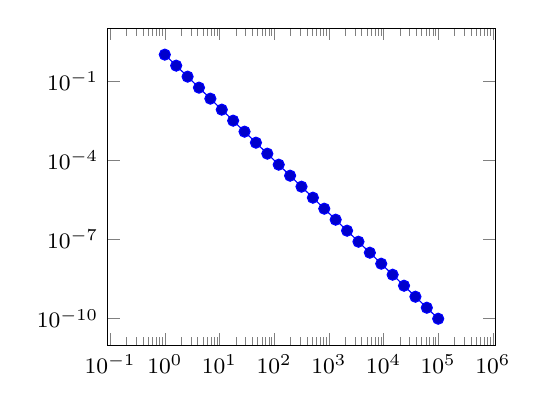
\begin{tikzpicture}
\begin{loglogaxis}[
    small,
    enlarge x limits={abs=11},
]
    \addplot+ [domain=1:100000] {x^-2};
\end{loglogaxis}
\end{tikzpicture}
\end{codeexample}

    请注意，|enlargelimits| 在将坐标轴界限的任何更改视为 |scale mode| 的一部分之前应用：|enlargelimits| 总是会被应用。之后，选项 |scale mode=scale uniformly| 将再次增大界限以满足所有缩放约束。这两次界限增大是相互独立的，即即使你设置 |enlargelimits=false|，如果看起来有必要，|scale mode| 仍会增大坐标轴界限。此规则的一个例外是按尺寸增大，即类似 |abs=1cm| 的情况（此情况请参阅 |enlargelimits respects figure size|）。有关如何禁用由 |scale mode| 引起的界限增大的详细信息，请参阅 |scale mode|（尤其是 |scale mode=units only|）和 |unit rescale keep size|。
\end{pgfplotsxykeylist}

\begin{pgfplotskey}{enlargelimits respects figure size=\mchoice{true,false} (initially true)}
    此键\emph{仅}用于类似 |enlarge x limits={abs=1cm}| 的情况，即按尺寸增大。它控制 \PGFPlots{} 是否会尝试遵守 |width|/|height|。除非遇到问题，否则你可能应该始终将其保留为默认值。

    如果 \PGFPlots{} 未能遵守图形尺寸，它将向日志文件打印一条类似 ``enlargelimits respects figure size=true: could not respect the prescribed width/height'' 的警告消息。
    \index{Errors!enlargelimits respects figure size=true: could not respect the prescribed width/height}
\end{pgfplotskey}

\begin{pgfplotsxykeylist}{%
    log origin \x=\mchoice{0,infty} (initially infty),
    log origin=\mchoice{0,infty} (initially infty)%
}
    允许选择哪个坐标是对数图的逻辑“原点”（针对某一坐标轴或所有坐标轴）。

    选项 |log origin=infty| 可能对堆叠图有用：它将对数坐标中的“原点”定义为 $-\infty$。为了与旧版本兼容，这是默认值。请注意，$-\infty$ 会被裁剪为相关坐标轴上显示的最低值。

    选项 |log origin=0| 将对数原点定义为自然选择 $\log(1)=0$。这对 |ycomb| 图特别有用。
\end{pgfplotsxykeylist}

\begin{pgfplotskey}{update limits=\mchoice{true,false} (initially true)}
    可用于中断数据界限的更新（例如，针对单个 |\addplot| 命令）。

    这与 |\pgfplotsinterruptdatabb| ... |\endpgfplotsinterruptdatabb| 具有相同的效果。
\end{pgfplotskey}

\begin{environment}{{pgfplotsinterruptdatabb}}
\index{Bounding Box Control!Disable \protect\emph{data} bounding box modifications}
    \meta{environment contents} 中的所有内容都不会对数据包围盒产生贡献。

    在花括号内使用 |update limits=false| 可以达到相同的效果。
\end{environment}


\subsection{访问计算出的界限范围}

本节面向那些想要或需要以编程方式访问计算出的界限的用户。它列出了如何访问计算出的值。

\begin{pgfplotsxykeylist}{\x min,\x max}
    这些值不仅是\emph{输入}：在探查阶段之后，它们的值将被计算出的结果值覆盖。这些值可能因 |enlargelimits| 或 |scale mode| 而不同。

    如果你需要访问它们，可以在代码中的某处写入 |\pgfkeysvalueof{/pgfplots/xmin}|。
\end{pgfplotsxykeylist}

%--------------------------------------------------
% \begin{pgfplotsxykeylist}{axis/zero/\x}
%     These values will be populated with the ``zero'' values of the respective axis. This zero value can differ from `$0$' due to either the configuration or programmatical usefulness:
%
%     \begin{itemize}
%         \item if the axis is linear and $0$ is part of the displayed limits, the key will expand to~$0$.
%         \item if the axis is linear but $0$ is outside of the displayed limits, the key will expand to the nearest point inside of the axis limits.
%         \item if the axis is logarithmic, the value will be set according to the |log origin| key and will be clipped to the displayed limits.
%     \end{itemize}
%
%     These keys are a property of the axis; they are unrelated to ``zero levels'' in the context of stacked plots.
% \end{pgfplotsxykeylist}
%--------------------------------------------------
